\documentclass[article]{jss}
\usepackage[utf8]{inputenc}

\author{
David L Miller\\University of St Andrews \And Jeffrey L Laake\\National Marine Mammal Laboratory
}
\title{Distance Sampling in \proglang{R}}
\Keywords{distance sampling, abundance estimation, line transects, point transects, \proglang{R}}

\Abstract{
The abstract of the article.
}

\Plainauthor{David L Miller, Jeffrey L Laake}
\Plaintitle{Distance Sampling in R}
\Plainkeywords{distance sampling, abundance estimation, line transects, point transects, R}

%% publication information
%% \Volume{50}
%% \Issue{9}
%% \Month{June}
%% \Year{2012}
\Submitdate{}
%% \Acceptdate{2012-06-04}

\Address{
    David L Miller\\
  University of St Andrews\\
  Centre for Research into Ecological and Environmental Modelling, The
  Observatory, St Andrews, Fife KY16 9LZ, Scotland\\
  E-mail: \href{mailto:dave@ninepointeightone.net}{\nolinkurl{dave@ninepointeightone.net}}\\
  URL: \url{http://converged.yt}\\~\\
      Jeffrey L Laake\\
  National Marine Mammal Laboratory\\
  Alaska Fisheries Science Center 7600 Sand Point Way N.E., Seattle, WA
  98115, USA\\
  E-mail: \href{mailto:Jeff.Laake@noaa.gov}{\nolinkurl{Jeff.Laake@noaa.gov}}\\
  
  }

\usepackage{amsmath} \usepackage{amssymb} \usepackage{longtable}
\usepackage{booktabs}

\begin{document}

\section{Introduction}\label{introduction}

Distance sampling (Buckland et al. 2001; Buckland et al. 2004)
encompases a suite of field methods and statistical models used to
estimate the abundance of biological populations. Distance sampling
field procedure can be thought of as an extension of plot sampling,
where we wish to take into account the decreasing probability of
detecting objects at increasing distance from the sampler. We do this by
building a model for detectability and use quantities calculated from
the detection function to adjust the observed counts to obtain an
estimate of abundance.

For many years distance sampling analyses have been available via the
Windows program Distance (or ``DISTANCE''); for clarity henceforth
``Distance for Windows'' Thomas et al. (2010)). From version 5 of
Distance for Windows, R packages have been included to perform
particular analyses (CITE Distance user manual). This paper shows how to
fit detection functions, perform model checking and selection and
estimate abundance in \proglang{R} using the package \pkg{Distance}.
\pkg{Distance} is a wrapper package around the more complex (and more
powerful) \pkg{mrds} and offers a subset of the analyses possible with
that package.

\subsection{Distance sampling}\label{distance-sampling}

Census-type surveys (quadrat or strip transects assuming perfect
detectability within strips or quadrats) are inefficient (requiring
considerable field effort) and we should expect that not all objects
(animals, plants, dung, etc) can be observed. Accounting for imperfect
detectability is an important consideration when obtaining accurate
estimates of abundance (Lahoz-Monfort, Guillera-Arroita, and Wintle
2013). Using the extra information gained by recording distance from the
sampler to the observation, it is possible to model detectability.
Because we expect detectability to decrease with increasing distance
from the sampler, we model detectability as a function of distance (plus
perhaps other covariates, see below). We use the probabilities of
detection calculated from the detection function to estimate an
abundance for the area covered by the survey, which we then scale-up to
the study region of interest.

Distance sampling surveys are conducted using two transect types: line
and point transects. In line transect sampling observers walk (or fly,
sail, etc) lines observing objects and recording the distances to the
line; whereas in point transect sampling observers remain stationary at
a location and record distances from that point. Field methods are
chosen to be suitable to species and habitat constraints (Buckland et
al. 2015).

\begin{CodeChunk}
\begin{figure}

{\centering 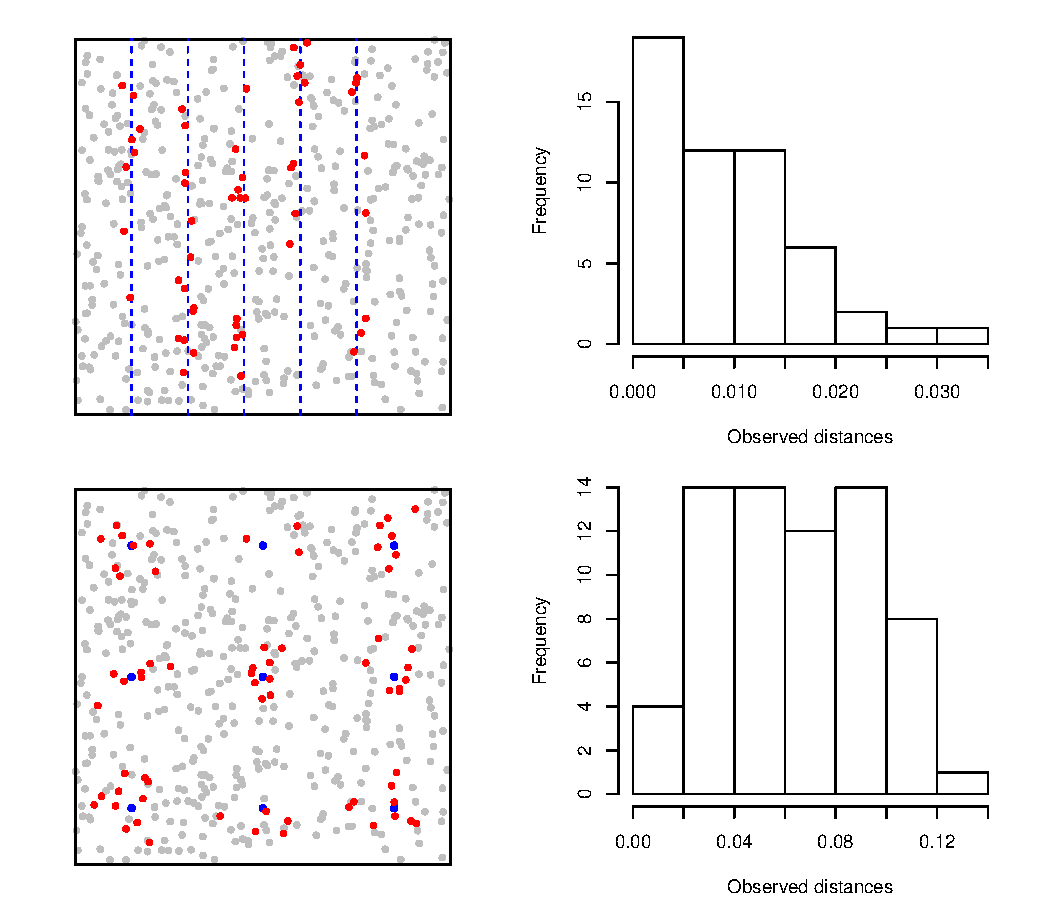
\includegraphics{paper_files/figure-latex/points-and-lines-1} 

}

\caption{Left side plots show an example of a survey of an area containing a population of 500 objects, blue indicates sampler placement (top lines, bottom points) and red dots indicate detected individuals. The right side of the figure shows histograms of observed distances (again, lines top and points bottom).\label{fig:pointslines}}\label{fig:points-and-lines}
\end{figure}
\end{CodeChunk}

For both points and lines, once the geometry of the sampler (see
``Detection functions'') has been taken into account, the histogram of
distances should show a decreasing number of observations with
increasing distance from the sampler. For line transects we expect
objects to be distributed unformly with respect to distance from the
line and what makes our histogram decrease is the detectability. For
point transects, we recognise that as distance from the point increases,
the area of the circle encompassed increases with distance squared;
hence the number of objects available to be detected is a linearly
increasing function of distance from the point.

Using this histogram we can crudely estimate the drop-off in
detectability by eye by tracing a line that approximates the tops of the
histogram bars -- this is the detection function. \pkg{Distance}
estimates the parameters for a fixed-form detection function using
maximum likelihood estimation. We address possible models in detail
below.

Figure \ref{fig:pointslines} shows examples of 500 individuals sampled
using line and point transects (left column) and their corresponding
histograms (right column).

\subsection{Data}\label{data}

We demonstrate \pkg{Distance} using two data sets: one line transect and
one point transect. These data sets have been chosen to be
representative of the kind of data seen in practice.

\subsubsection{Minke whales}\label{minke-whales}

The line transect data is simulated data based on a survey of Antarctic
minke whales (\emph{Balaenoptera bonaerensis}). The data is simulated
from models fitted to data from the International Whaling Commission's
International Decade of Cetacean Research Southern Ocean Whale and
Ecosystem Research (IWC IDCR-SOWER) programme 1992-1993 austral summer
surveys (Branch and Butterworth 2001). They consist of 99 observations
and include information on the effort expended and whether observations
were in one of two geographical strata (near or far from land).

\subsubsection{Amakihi}\label{amakihi}

The point transect data set consists of 1485 observations of Amakihi
(\emph{Hemignathus virens}; a Hawaiian songbird), collected at 41 points
between 1992 and 1995. The data include distances and three covariates
collected during the survey: observer ID (a three level factor), minutes
after sunrise (continuous) and hours after sunrise (a six level factor).
Data are analysed comprehensively in Marques et al. (2007).

\subsection{The rest of the paper}\label{the-rest-of-the-paper}

The rest of the paper has this structure: we describe data organisation
for use with \pkg{Distance}; models for the detection function are
described in terms of formulation and examples of fitting in
\proglang{R}. We then examine model checking, goodness of fit and model
selection. Having illustrated how to obtain a good detection function,
we show how to estimate abundance using that model, including
stratification. The final two sections of the article look at extensions
(both in terms of methodology and software) and put the package in a
broader context amongst other software packages used for estimating the
abundance of biological populations.

\section{Data setup}\label{data-setup}

The two example data sets used here are distributed with \pkg{Distance}
so readers can reproduce our results. However, data will be collected in
the field and formatted correctly for use with \pkg{Distance}. The
package allows for a flexible format for data input ranging from very
simple to complex:

\begin{itemize}
\itemsep1pt\parskip0pt\parsep0pt
\item
  In the simplest case, where one would simply like to estimate a
  detection function, all that is needed is a vector of distances.
\item
  To include additional covariates into the detection function (see
  ``Detection functions'') we need to use a \code{data.frame}. The
  data.frame contains a column called \code{distance} and additional
  named columns for covariates potentially useful in modelling
  detectability (for example \code{observer} or \code{seastate}). Some
  column names are reserved: \code{object} for an observation identifier
  (see ``Extensions''), \code{size} for group or cluster size (see
  ``Detection functions'' and ``Abundance and variance estimation''),
  \code{detected} for whether an observation was detected (see
  ``Extensions'') and the columns described in the next bullet.
\item
  If one would like to estimate abundance beyond area covered by
  expended survey effort, additional information is required. This
  consists of information about which transect and occasion the
  observation was made (the \code{Sample.Label}), a column named
  \code{Effort} which gives the effort associated with that sample (for
  lines their length and for points the number of times that point was
  visited), the stratum the sample was located in (this may have any
  name and may be from pre- or post-survey stratification, see
  ``Estimating abundance and variance'') and that stratum's area (which
  has the same name as the stratum column, appended with \code{.Area}).
  (We refer to this data format as ``flatfile'' where all information is
  contained in one table.)
\end{itemize}

As we will see in ``Extensions'', further information is also required
when we start using more complex models.

The minke whale data follows the ``flatfile'' format given in the last
bullet point:

\begin{CodeChunk}
\begin{CodeInput}
library(Distance)
head(minke)
\end{CodeInput}
\begin{CodeOutput}
  Region.Label  Area Sample.Label Effort distance
1        South 84734            1  86.75     0.10
2        South 84734            1  86.75     0.22
3        South 84734            1  86.75     0.16
4        South 84734            1  86.75     0.78
5        South 84734            1  86.75     0.21
6        South 84734            1  86.75     0.95
\end{CodeOutput}
\end{CodeChunk}

Whereas the amakihi data lacks effort and stratum data:

\begin{CodeChunk}
\begin{CodeInput}
head(amakihi)
\end{CodeInput}
\begin{CodeOutput}
   survey object distance obs mas has detected
1 July 92      1       40 TJS  50   1        1
2 July 92      2       60 TJS  50   1        1
3 July 92      3       45 TJS  50   1        1
4 July 92      4      100 TJS  50   1        1
5 July 92      5      125 TJS  50   1        1
6 July 92      6      120 TJS  50   1        1
\end{CodeOutput}
\end{CodeChunk}

We'll explore what the effects of including effort data are during
analysis below.

\section{Detection functions}\label{detection-functions}

As mentioned above, the detection function describes the relationship
between observed distances and probability of detection. The detection
function itself models the probability
\(\mathbb{P}(\text{object detected } \vert \text{ object at distance } y)\)
and is usually denoted \(g(y; \boldsymbol{\theta})\) where \(y\) is
distance (either from a line or point) and \(\boldsymbol{\theta}\) is a
vector of parmeters to be estimated. Our goal is to estimate an
\emph{average probability of detection} (\(p\), average in the sense of
an average over the distances), so we must integrate out distance
(\(y\)) from the detection function: \[
p = \int_0^w \pi(y) g(y; \boldsymbol{\theta}) dy
\] where \(\pi(y)\) describes the distribution of objects with respect
to the sampler and \(\pi(x)=1/w\) for line transects and
\(\pi(r)=\frac{2r}{w^2}\) for point transects, taking into account the
geometry of the sampler (Buckland et al. 2001, Chapter 3) (letting \(x\)
denote a perpendicular distance from a line and \(r\) denote radial
distance from a point).

It is important that the detection function accurately models
detectability near zero distance. We are less worried by its behaviour
further away from 0. To ensure that the model is not overly influence by
distances far from zero we truncate the distances beyond a given
distance \(w\) (known as the \emph{truncation distance}). Fitting to
distances at great distances from zero does not demonstrably improve the
precision of abundance estimates (Buckland et al. 2001, 103--8,
151--53).

Models for the detection function are expected to have the following
properties (Buckland et al. 2015, Chapter 5):

\begin{itemize}
\itemsep1pt\parskip0pt\parsep0pt
\item
  \emph{Shoulder}: we expect observers to be able to see objects near
  them, not just those directly infront of them. For this reason, we
  expect the detection function to be ``flat'' near zero distance.
\item
  \emph{Non-increasing}: we don't think that observers should be more
  likely to see things further away than those nearer to them. This
  usually indicates an issue with field procedure (that the distribution
  of objects with respect to the line, \(\pi(y)\) is not what we
  expect), so we do not want the detection function to model this.
\item
  \emph{Model robust}: models should be flexible enough to make many
  different shapes.
\item
  \emph{Pooling robust}: many factors can affect the probability of
  detection and it is not possible to measure all of these. We would
  like our models to be robust to us not including these factors.
\item
  \emph{Estimator efficiency}: we would like our models to have low
  variances, but only given they satisfy the other properties above
  (which, if they are satisfied, would give low bias).
\end{itemize}

Given these criteria, we can start to think about models for \(g\).

\subsection{Formulations}\label{formulations}

There is a wide literature on possible formulations for the detection
function (Buckland 1992; Eidous 2005; Becker and Quang 2009; Giammarino
and Quatto 2014; Miller and Thomas 2015; Becker and Christ 2015).
\code{Distance} includes the most popular of these models. Here we'll
detail the most popular detection function approach: ``key function plus
adjustments'' (K+A).

\subsubsection{Key function plus adjustments
(K+A)}\label{key-function-plus-adjustments-ka}

Key function plus adjustment terms (or adjustment series) models are
formulated by taking a ``key'' function and optionally adding
``adjustments'' to it to improve the fit (Buckland 1992). Mathematically
we formulate this as: \[
g(y; \boldsymbol{\theta}) = k(y; \boldsymbol{\theta}_\text{key})\left( 1+ \alpha_O(y; \boldsymbol{\theta}_\text{adjust})\right),
\] where \(k\) is the key function and \(\alpha_O\) is sum series of
functions (given in Table \ref{tab:keyadj}), described as an
\emph{adjustment of order \(O\)}. Subscripts on the parameter vector
indicate those parameters belonging to each part of the model (i.e.
\(\boldsymbol{\theta} = (\boldsymbol{\theta}_\text{key}, \boldsymbol{\theta}_\text{adjust})\)).

Available models for the key are as follows: \[
k(y) = \left\{
\begin{array}{l l}
  \exp\left(-\frac{y^2}{2 \sigma^2}\right) & \quad \text{half-normal,} \\
  1-\exp\left(\left(-\frac{y}{\sigma}\right)^{-b}\right) & \quad \text{hazard-rate,} \\
  1/w & \quad \text{uniform.}
\end{array} \right.
\] Possible modelling options for key and adjustments are given in Table
\ref{tab:keyadj} and illustrated in Figure \ref{fig:hnhr} and
\ref{fig:keyadj}. We select the number of adjustment terms (\(K\)) by
AIC (further details in ``Model checking and model selection'').

\begin{CodeChunk}
\begin{figure}

{\centering 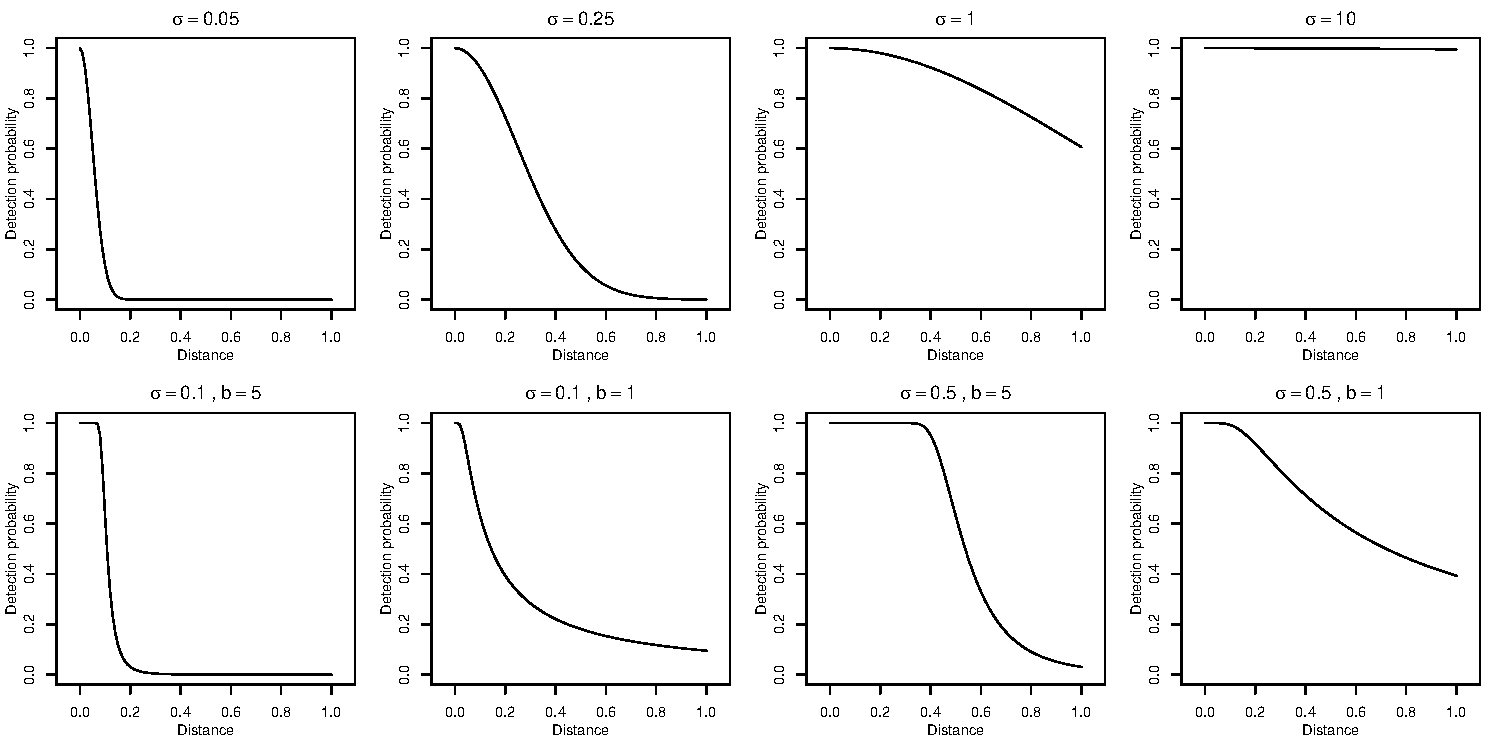
\includegraphics{paper_files/figure-latex/hn-hr-par-comp-1} 

}

\caption{Half-normal (top row) and hazard-rate (bottom row) detection functions without adjustments, varying scale ($\sigma$) and (for hazard-rate) shape ($b$) parameters (values are given above the plots). On the top row from left to right, the study species becomes more detectable (higher probability of detection at larger distances). The bottom row shows the hazard-rate model's more pronounced shoulder.\label{fig:hnhr}}\label{fig:hn-hr-par-comp}
\end{figure}
\end{CodeChunk}

\begin{table}
\caption{Modelling options for key plus adjustment series models for the detection function.}
\begin{tabular}{llll}
\hline
Key function   & Form   & Adjustment series & Form\\
\hline
 Uniform  & $1/w$   & cosine  & $\sum_{o=1}^O a_o \cos(o \pi y/w)$ \\
 & & Simple polynomial & $\sum_{o=1}^O a_o (y/w)^{2o}$ \\
 Half-normal  & $\exp\left(-\frac{y^2}{2 \sigma^2}\right)$ & cosine  & $\sum_{o=2}^O a_o \cos(o \pi y/w)$ \\
 & & Hermite polynomial & $\sum_{o=2}^O a_o H_{2o}(y/\sigma)$ \\
 Hazard-rate  & $1-\exp\left[-\left(\frac{y}{\sigma}\right)^{-b}\right]$ & cosine  & $\sum_{o=2}^O a_o \cos(o \pi y/w)$ \\
 & & Simple polynomial & $\sum_{o=2}^O a_o (y/w)^{2o}$ \\
\hline
\end{tabular}
\label{tab:keyadj}
\end{table}

When adjustment terms are used it may be necessary to standardise the
results to ensure that \(g(0)=1\), so we can redefine the detection
function as: \[
g(y; \boldsymbol{\theta}) = \frac{k(y; \boldsymbol{\theta}_\text{key})\left( 1+ \alpha_O(y; \boldsymbol{\theta}_\text{adjust})\right)}{k(0; \boldsymbol{\theta}_\text{key})\left( 1+ \alpha_O(0; \boldsymbol{\theta}_\text{adjust})\right)}.
\]

A disadvantage of K+A models is that we must resort to constrained
optimisation (via the \pkg{Rsolnp} package) in order to ensure that the
resulting detection function is monotonic non-increasing over the whole
range.

We do not always include adjustments (except in the case of the uniform
key), in which case we refer to ``key only'' models (see the next
section and ``Model checking and model selection'').

\begin{CodeChunk}
\begin{figure}

{\centering 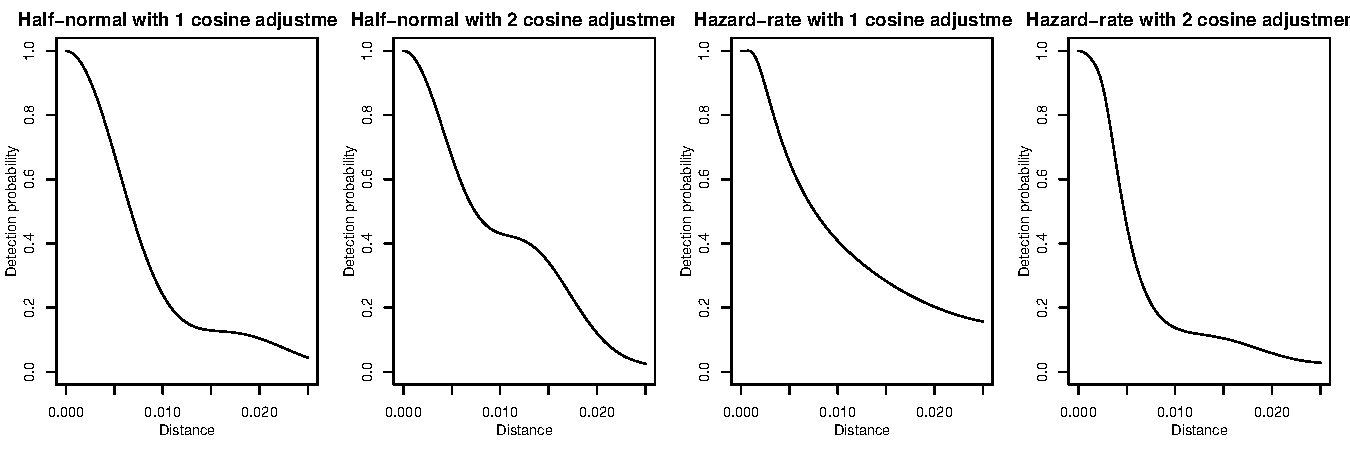
\includegraphics{paper_files/figure-latex/adjust-mix-comp-1} 

}

\caption{Possible shapes for the detection function when adjustments are included for half-normal and hazard-rate models.\label{fig:keyadj}}\label{fig:adjust-mix-comp}
\end{figure}
\end{CodeChunk}

\subsubsection{Covariates}\label{covariates}

There are many factors that can affect the probability of detecting an
object. These include things like the observer, the vessel or platform
used, the sea state, weather conditions and time of day (to name but a
few). We assume that these variables affect detection only via the scale
of the detection function (and do not affect the shape).

Covariates can be included in this formulation by considering the scale
parameter from the half-normal or hazard-rate detection functions as a
linear model (on the exponential scale) of the (\(J\)) covariates
(\(\mathbf{z}\); a vector of length \(J\) for each observation): \[
\sigma(\mathbf{z}) = \exp(\beta_0 + \sum_{j=1}^J \beta_j z_j).
\] In the next section we'll discuss model selection.

Including covariates has an important implication for our calculation of
detectability. Since we don't know what the true distribution of the
covariates is we must calculate the probability of detection conditional
on the observed values of the covariates: \[
p(\mathbf{z_i}) = \int_0^w \pi(y) g(y, \mathbf{z_i}; \boldsymbol{\theta}) dy,
\] where \(\mathbf{z_i}\) is the vector of \(J\) covariates associated
with observation \(i\). So for covariate models, we are calculating a
value of ``average'' probability of detection (again the average is in
the sense of distance) per observation. There will be as many unique
values of \(p(\mathbf{z_i})\) as there are unique covariate combinations
in our data.

Another important consideration is that K+A models which include
covariates and one or more adjustments cannot be guaranteed to be
monotonic non-increasing for all covariate combinations, as we don't
have any model for the distribution of the covariates. For this reason,
we advise against using both adjustments and covariates in a detection
function (see Miller and Thomas 2015 for an example of when this can be
problematic).

\subsection{Fitting detection functions in
R}\label{fitting-detection-functions-in-r}

The workhorse of detection function fitting in \pkg{Distance} is the
\code{ds} function. Here we show off the formulations for the detection
function that we've seen above for both the minke whale and amakihi
data.

\subsubsection{Minke whale}\label{minke-whale}

We can fit a model to the minke whale data, setting the truncation at
1.5km and using the default options in \code{ds} very simply:

\begin{CodeChunk}
\begin{CodeInput}
minke_hn <- ds(minke, truncation=1.5)
\end{CodeInput}
\begin{CodeOutput}
Starting AIC adjustment term selection.
Fitting half-normal key function
Key only models do not require monotonicity contraints. Not constraining model for monotonicity.
AIC= 46.872
Fitting half-normal key function with cosine(2) adjustments
AIC= 48.872


half-normal key function selected!
\end{CodeOutput}
\end{CodeChunk}

Note that \code{ds} will automatically select adjustment terms by AIC
and shows it's selection steps as it goes.

Figure \ref{fig:minkeamakihi} (top left plot) shows the result of
calling \code{plot} on the resulting model object. We can also call
\code{summary} on the model object to get summary information about the
fitted model (though we postpone this until the next section).

We can specify the form of the detection function via the \code{key=}
argument to \code{ds}. For example, a hazard rate model can be fitted
as:

\begin{CodeChunk}
\begin{CodeInput}
minke_hrcos <- ds(minke, truncation=1.5, key="hr")
\end{CodeInput}
\begin{CodeOutput}
Starting AIC adjustment term selection.
Fitting hazard-rate key function
Key only models do not require monotonicity contraints. Not constraining model for monotonicity.
AIC= 48.637
Fitting hazard-rate key function with cosine(2) adjustments
AIC= 50.386


hazard-rate key function selected!
\end{CodeOutput}
\end{CodeChunk}

Again, \code{ds} fits a model with cosine adjustments (the default) but
finds the AIC improvement to be insufficient to select the adjustment.

\subsubsection{Amakihi}\label{amakihi-1}

By default \code{ds} assumes that the data given to it is line transect,
but we can switch to points using \code{transect="point"}. Including
covariates in the scale is via the \code{formula=~...} argument to
\code{ds}; a hazard-rate model for the amakihi that includes observer as
a covariate can be specified by (truncating at 82.5m, given in Marques
et al. 2007):

\begin{CodeChunk}
\begin{CodeInput}
amakihi_hr_obs <- ds(amakihi, truncation=82.5, transect="point",
                     key="hr", formula=~obs)
\end{CodeInput}
\begin{CodeOutput}
Cannot perform AIC adjustment term selection when covariates are used.
Fitting hazard-rate key function
AIC= 10778.448
No survey area information supplied, only estimating detection function.
\end{CodeOutput}
\end{CodeChunk}

As with the minke whale model, we can plot the resulting detection
function (Figure \ref{fig:minkeamakihi}, centre column). Since for the
amakihi we used covariates in the detection function, the plot will show
the detection function averaged over levels/values of the covariate.
Points on the plot indicate probability of detection for each
observation. For the \texttt{amakihi\_hr\_obs} model we see fairly clear
levels of the observer covariate in the points. Looking at the left
panel of Figure \ref{fig:minkeamakihi}, we can see this is less clear
when adding minutes after sunrise as a covariate into the model:

\begin{CodeChunk}
\begin{CodeInput}
amakihi_hr_obs_mas <- ds(amakihi, truncation=82.5, transect="point",
                         key="hr", formula=~obs+mas)
\end{CodeInput}
\begin{CodeOutput}
Cannot perform AIC adjustment term selection when covariates are used.
Fitting hazard-rate key function
AIC= 10777.376
No survey area information supplied, only estimating detection function.
\end{CodeOutput}
\end{CodeChunk}

The bottom row of Figure \ref{fig:minkeamakihi} shows the probability
density functions for the amakihi models. These often are easier to
interpret than the detection functions, as for point data we must
rescale the histogram when plotting the detection function to take into
account the geometry of the point sampler.

\begin{CodeChunk}
\begin{figure}

{\centering 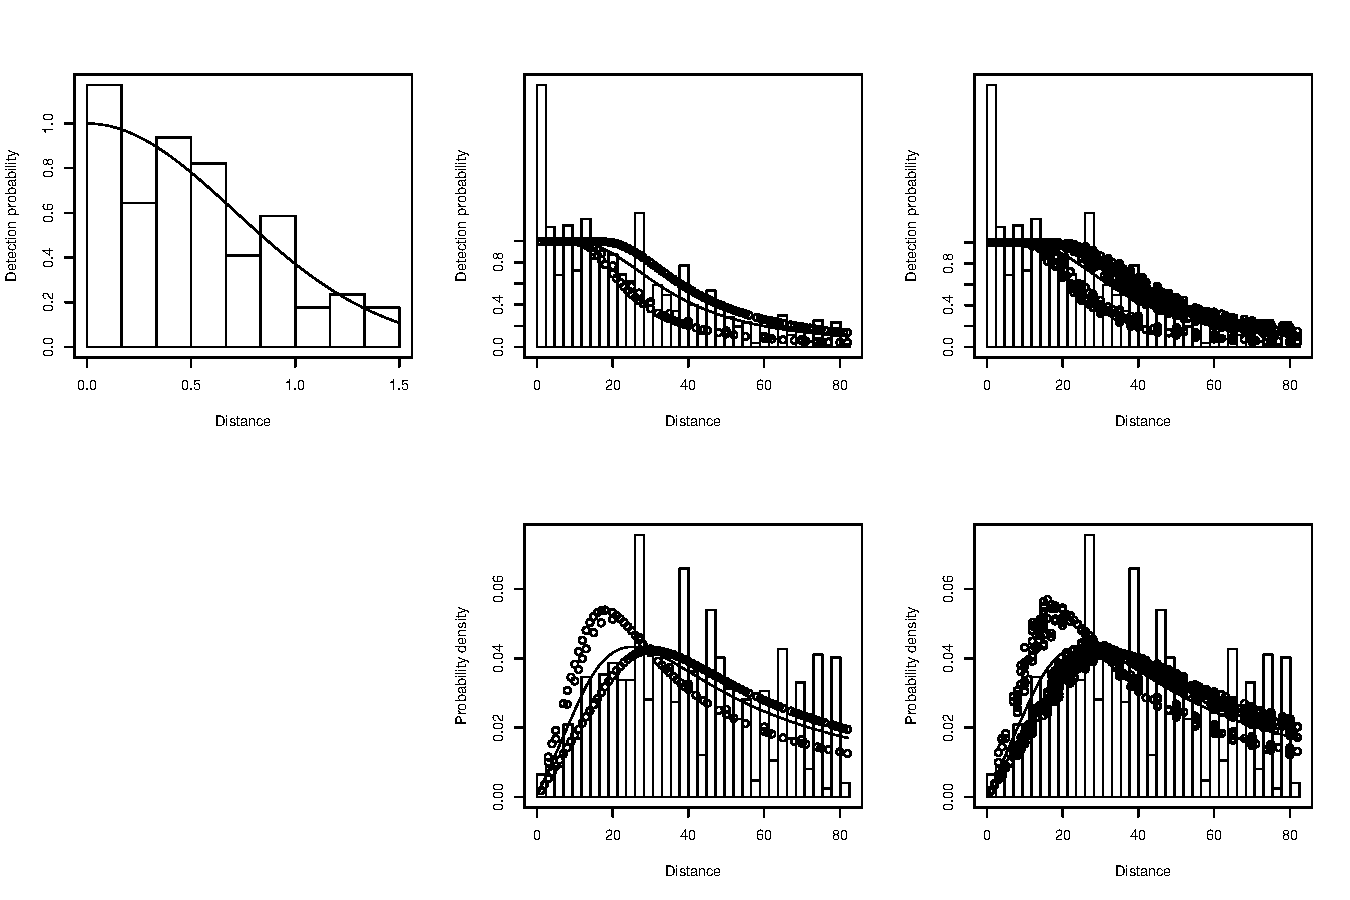
\includegraphics{paper_files/figure-latex/minke-amakihi-hn-plot-1} 

}

\caption{Top row plots of fitted detection functions overlayed on the histograms of observed distances; left minke whale data, half-normal model; centre, amakihi data hazard-rate with observer as a covariate; right, amakihi data, hazard-rate model with observer and minutes after sunrise as covariates (for amakihi histograms are rescale to take into account sampler geometry). Bottom row shows plots of the probability density function for the amakihi models (as top row). For covariate models (centre and right columns) points indicate probability of detection for a given observation (given that observations covariate values) and lines indicate the average detection function.\label{fig:minkeamakihi}}\label{fig:minke-amakihi-hn-plot}
\end{figure}
\end{CodeChunk}

\section{Model checking and model
selection}\label{model-checking-and-model-selection}

As with models fitted using \code{lm} or \code{glm} in \proglang{R}, we
can use \code{summary} to give us some useful information about our
fitted model. For example for our hazard-rate model for the amakihi,
with observer as a covariate:

\begin{CodeChunk}
\begin{CodeInput}
summary(amakihi_hr_obs)
\end{CodeInput}
\begin{CodeOutput}

Summary for distance analysis 
Number of observations :  1243 
Distance range         :  0  -  82.5 

Model : Hazard-rate key function 
AIC   : 10778.45 

Detection function parameters
Scale coefficient(s):  
              estimate         se
(Intercept) 3.06441705 0.10878121
obsTJS      0.53017364 0.09956539
obsTKP      0.08885471 0.18071851

Shape coefficient(s):  
             estimate         se
(Intercept) 0.8690009 0.06261764

                        Estimate          SE         CV
Average p              0.3142723   0.0204413 0.06504326
N in covered region 3955.1685709 274.2284029 0.06933419
\end{CodeOutput}
\end{CodeChunk}

This summary information includes various details of the data and model
specification, as well as the values of the coefficents (\(\beta_j\))
and their uncertainties, an ``average'' value for the detectability (see
``Estimating abundance and variance'' for details on how this is
calculated) and it's uncertainty. The final line gives an estimate of
abundance for the area covered by the survey (again, this will be
covered in detail in the next section).

\subsection{Goodness of fit}\label{goodness-of-fit}

To judge goodness of fit for detection functions when exact distances
are used, we want to compare the cumulative distribution function (CDF)
and empirical distribution function (EDF) for the detection function via
a quantile-quantile plot (Q-Q plot). In our case the CDF evaluates the
probability of observing an object at a distance less than or equal to
some given value. The EDF gives the proportion of observations for which
the CDF is less than or equal to that of a given distance. In essence
we're asking ``is the number of observations up to a given distance in
line with what the model says they should be?'' (where `given values'
are the observed distances). As usual for Q-Q plots, ``good'' models
will have values close to the line \(y=x\), poor models will show more
deviations from that line.

We can inspect Q-Q plots visually, though for a large number of models
this can be tiresome and prone to subjective judgements. Instead we can
quantify the Q-Q plot's information using a Kolmogorov-Smirnov or
Cramer-von Mises test (Burnham et al. 2004). Both test to see if the
points from the EDF and CDF are from the same distribution. The
Kolmogorov-Smirnov uses the test statistic of the largest difference
between a point on the Q-Q plot and the line \(y=x\), whereas the
Cramer-von Mises test uses the sum of all the differences. As it takes
into account more information and is therefore more powerful, the
Cramer-von Mises is generally preferred. A significant result from
either tests indicates that the EDF and CDF do not come from the same
distribution (and therefore the model is does not fit the data well).

We can generate a Q-Q plot and test results using the \code{gof_ddf}
function. We can see the goodness of fit tests below for two models for
the amakihi data, first fitting a half-normal model without covariates
or adjustments (not setting \code{adjustment=NULL} will force \code{ds}
to fit a model with no adjustments), then calculating goodness of fit
for that model and our hazard-rate model with observer and minutes after
sunrise included:

\begin{CodeChunk}
\begin{CodeInput}
amakihi_hr <- ds(amakihi, truncation=82.5, transect="point", key="hn", adjustment=NULL)
\end{CodeInput}
\begin{CodeOutput}
Fitting half-normal key function
Key only models do not require monotonicity contraints. Not constraining model for monotonicity.
AIC= 10833.841
No survey area information supplied, only estimating detection function.
\end{CodeOutput}
\begin{CodeInput}
gof_ds(amakihi_hr)
\end{CodeInput}
\begin{CodeOutput}

Goodness of fit results for ddf object

Distance sampling Kolmogorov-Smirnov test
Test statistic =  0.059345  P =  0.00031527 

Distance sampling Cramer-von Mises test (unweighted)
Test statistic =  0.93083  P =  0.003578 
\end{CodeOutput}
\begin{CodeInput}
gof_ds(amakihi_hr_obs_mas)
\end{CodeInput}
\begin{CodeOutput}

Goodness of fit results for ddf object

Distance sampling Kolmogorov-Smirnov test
Test statistic =  0.036251  P =  0.076237 

Distance sampling Cramer-von Mises test (unweighted)
Test statistic =  0.15016  P =  0.38908 
\end{CodeOutput}
\end{CodeChunk}

The corresponding Q-Q plots are shown in Figure \ref{amakihi-qq}.

\begin{CodeChunk}
\begin{figure}

{\centering 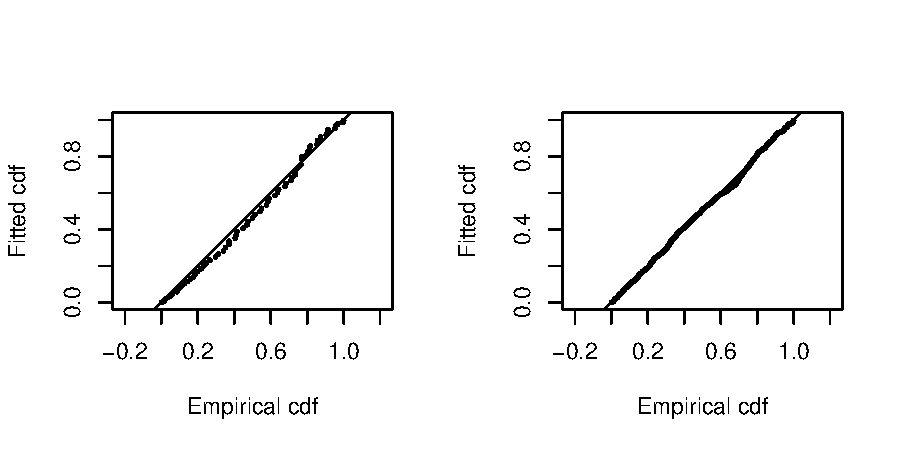
\includegraphics{paper_files/figure-latex/amakihi-qq-comp-1} 

}

\caption[Comparison of quantile-quantile plots for a half-normal model (no adjustments, no covariates) and hazard-rate model with observer and minutes after sunrise for the amakihi data]{Comparison of quantile-quantile plots for a half-normal model (no adjustments, no covariates) and hazard-rate model with observer and minutes after sunrise for the amakihi data.\label{amakihi-qq}}\label{fig:amakihi-qq-comp}
\end{figure}
\end{CodeChunk}

\subsection{Model selection}\label{model-selection}

Once we have a set of models which fit well, we can use Akaike's
Information Criterion (AIC) to select between models. \pkg{Distance}
includes a function to create table of summary information for fitted
models, making it easy to get an overview of a large number of models at
once. The \code{summarize_ds_models} function takes models as input and
can be especially useful when paired with \pkg{knitr}'s \code{kable}
function to create summary tables for publication. An example of this
output is shown in Table \ref{tab:amakihi} and was generated by:

\begin{CodeChunk}
\begin{CodeInput}
library(knitr)
summarize_ds_models(amakihi_hr, amakihi_hr_obs, amakihi_hr_obs_mas)
\end{CodeInput}
\end{CodeChunk}

\begin{table}

\caption{Summary for the detection function models fitted to the amakihi data. ``C-vM'' stands for Cramer-von Mises, $P_a$ indicates average detectability (see ``Estimating abundance and variance''), se indicates standard error. Models are sorted according to AIC.\label{tab:amakihi}}
\begin{tabular}{llrrrrr}
\toprule
Key function & Formula & C-vM $p$-value & $\hat{P_a}$ & se($\hat{P_a}$) & AIC & $\Delta$AIC\\
\midrule
Hazard-rate key function & ~obs + mas & 0.389 & 0.319 & 0.020 & 10777.38 & 0.000\\
Hazard-rate key function & ~obs & 0.271 & 0.314 & 0.020 & 10778.45 & 1.073\\
Half-normal key function & ~1 & 0.004 & 0.351 & 0.011 & 10833.84 & 56.465\\
\bottomrule
\end{tabular}
\end{table}

\section{Estimating abundance and
variance}\label{estimating-abundance-and-variance}

Though fiting the detection function is the primary modelling step in
distance sampling, we are really interested in estimating detectability,
and from that abundance. We also wish to calculate our certainty in each
abundance estimate. This section addresses these issues mathematically
before showing how to estimate abundance and its variance in R.

\subsection{Abundance}\label{abundance}

We wish to obtain the abundance in a study region, of which we have
sampled a (representative) subset. To do this we first calculate the
abundance in the area we have surveyed (the \emph{covered area}) to
obtain \(\hat{N}_\text{C}\), we can then scale this up to the full study
area by multiplying it by the ratio of covered area to study area.

First, in order to estimate abundance in the covered area
(\(\hat{N}_\text{C}\)), we use the estimates of detection probability
(the \(\{p_i; i=1,\ldots,n\}\), above) in a Horvitz-Thompson like
estimator:

\begin{equation}
\hat{N}_\text{C} = \sum_{i=1}^n\frac{s_i}{\hat{p}_i},
\label{ht}
\end{equation}

where \(s_i\) are the sizes of the observed groups of objects, which is
equal to 1 if objects only occur singly (Borchers and Burnham 2004).
Thompson (2002) is the cannonical reference to this type of estimator;
intuitively, we can think of the estimates of detectability
(\(\hat{p}_i\)) as ``inflating'' the group sizes (\(s_i\)) to account
for incomplete detection -- we then sum to obtain the abundance
estimate. For models that do not include covariates, \(\hat{p}_i\) is
equal for all \(i\), so this is equivalent to summing the groups and
inflating that sum by the corresponding
\(\hat{p} (=\hat{p}_i \forall i)\).

Having obtained the abundance in the covered area, we can then scale-up
to the study area: \[
\hat{N} = \frac{A}{a} \hat{N}_\text{C},
\] where \(A\) is the area of the study region to extrapolate the
abundance estimate to and \(a\) is the covered area. For line transects
\(a=2wL\) (twice the truncation distance multiplied by the total length
of transects surveyed) and for points \(a=\pi w^2 K\).

We can use the Horvitz-Thompson-like estimator to calculate the
``average'' detectability for models which include covariates. We can
consider what single detectability value would give the estimated
\(\hat{N}\) and therefore calculate: \[
\hat{P_a} = n/\hat{N}_\text{C}.
\] This can be a useful summary statistic and is included in the
\code{summary} output and the table produced by
\code{summarize_ds_models}.

\subsubsection{Stratification}\label{stratification}

We may wish to calculate abundance estimates for some sub-regions of the
study region, we call these areas \emph{strata}. A stratum may be
defined by, for example, a different habitat type or by the sex of the
animal (or some combination) which may be of interest for biological or
management reasons. In order to calculate estimates for a given
stratification each observation must occur in a stratum which must be
labelled with a \code{Region.Label} and have a corresponding \code{Area}
(if we are using an animal characteristic like sex, we would have the
areas be the same but if we were using say forested vs.~wetland habitat
the areas of those strata would be different). Finally, we must also
know which stratum a given transect lies in.

As an example the minke whale data consists of two strata: \code{North}
and \code{South} relating to a stratum further away and nearer the
Antarctic ice edge, respectively. Figure \ref{fig:minke-strata} shows
the two strata, along with observations and transect lines.

\begin{figure}
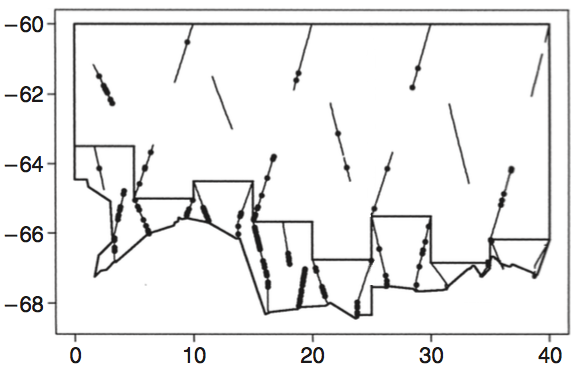
\includegraphics{minke-strata}
\label{fig:minke-strata}
\caption{Strata used for the minke whale data adapted from @Hedley:2004et. Points show the locations of observations along transect lines. The stepped line shows the boundary between North and South strata. Further details on the survey are available in @Branch:2001ua (simulated data is based on ``1992/93 Area III'' therein).}
\end{figure}

\subsection{Variance}\label{variance}

Here we take an intuitive approach to uncertainty estimation, for a full
derivations consult F. F. C. Marques and Buckland (2003). Uncertainty in
\(\hat{N}\) comes from two sources:

\begin{enumerate}
\def\labelenumi{\arabic{enumi}.}
\itemsep1pt\parskip0pt\parsep0pt
\item
  \emph{Model uncertainty}, from the estimation of the detection
  function parameters \(\boldsymbol{\theta}\)
\item
  \emph{Sampling uncertainty}, from the distribution of objects along
  the transect lines or between visiting occasions for points.
\end{enumerate}

We can see this by looking at the Horvitz-Thompson estimation in
(\ref{ht}) and consider the terms which are random. These are: the
detectability \(\hat{p}_i\) (and hence the parameters of the detection
function it is derived from) and \(n\), the number of observations. We
assume that the observed group size (\(s_i\)) is recorded without error.

Model uncertainty can be addressed using standard maximum likelihood
theory. We can invert the Hessian matrix of the likelihood to obtain a
variance-covariance matrix. We can then pre- and post-multiply this by
the derivatives of \(\hat{N}_\text{C}\) \[
\widehat{\text{Var}}_\text{model}\left( \hat{N}_\text{C}\right) = \left(\frac{\partial \hat{N}_\text{C}}{\partial\hat{\boldsymbol{\theta}}}\right)^\text{T} \left(\hat{\mathbf{H}}(\hat{\boldsymbol{\theta}})^{-1} \right)\frac{\partial \hat{N}_\text{C}}{\partial\hat{\boldsymbol{\theta}}}
\] where the partial derivatives of \(\hat{N}_\text{C}\) are evaluated
at the MLE (\(\hat{\theta}\)) and \(\mathbf{H}\) is the first partial
Hessian (outer product of first derivatives of the log likelihood) for
numerical stability (Buckland et al. 2001, p 62). Note that although we
calculate uncertainty in \(\hat{N}_\text{C}\), we can trivially scale-up
to variance of \(\hat{N}\).

Sampling uncertainty can be characterised (rather than as simply \(n\))
by the \emph{encounter rate}: the number of objects per unit transect.
When covariates are not included in the detection function we can define
the encounter rate as \(n/L\) for line transects (where \(L\) is the
total line length) or \(n/T\) for point transects (where \(T\) is the
total number of visits to all points). When covariates are included in
the detection function, it is recommended that we substitute the \(n\)
in the previous expressions with the estimated abundance \(\hat{N}\) as
this will take into account the effects of the covariates.

For line transects, by default, \pkg{Distance} uses a variation of the
estimator ``R2'' from Fewster et al. (2009) replacing number of
observations per sample with the estimated abundance per sample (Innes
et al. 2002; F. F. C. Marques and Buckland 2003): \[
\widehat{\text{Var}}_{\text{encounter},R2} = \frac{K}{L^2(K-1)} \sum_{k=1}^{K} l_k^2 \left( \frac{N_k}{l_k} - \frac{N}{L}\right)^2,
\] where \(l_k\) are the lengths of the \(K\) transects (such that
\(L = \sum_{k=1}^K l_k\)). Whereas for points we use estimator ``P3''
from Fewster et al. (2009) but again replacing \(n\) by \(\hat{N}\) to
obtain the following estimator: \[
\widehat{\text{Var}}_{\text{encounter},P3} = \frac{1}{T(K-1)} \sum_{k=1}^{K} t_k \left( \frac{N_k}{t_k} - \frac{N}{T}\right)^2,
\] where \(t_k\) is the number of visits to point \(k\) and
\(T = \sum_{k=1}^K t_k\).

Various formulations for the encounter rate variance are discussed in
detail in Fewster et al. (2009). \pkg{Distance} implements all of the
estimators of encounter rate variance given in that article. The
\code{varn} manual page gives further advice and technical detail on
encounter rate variance.

We combine these two sources of variance by noting that squared
coefficients of variation (approximately) add (Goodman 1960).

\subsection{Estimating abundance and variance in
R}\label{estimating-abundance-and-variance-in-r}

Going back to the minke whale data, we have the information we require
to calculate \(A\) and \(a\) above, so we can estimate abundance and its
variance. When we supply data to \code{ds} in the ``flatfile'' format
given above, \code{ds} will automatically calculate abundance estimates
based on the survey setup in the data.

Having already fitted a model to the minke whale data, we can see the
results of the abundance estimation by simply looking at a model
summary:

\begin{CodeChunk}
\begin{CodeInput}
summary(minke_hn)
\end{CodeInput}
\begin{CodeOutput}

Summary for distance analysis 
Number of observations :  88 
Distance range         :  0  -  1.5 

Model : Half-normal key function 
AIC   : 46.87216 

Detection function parameters
Scale coefficient(s):  
              estimate        se
(Intercept) -0.3411766 0.1070304

                       Estimate          SE         CV
Average p             0.5733038  0.04980421 0.08687229
N in covered region 153.4962706 17.08959835 0.11133559

Summary statistics:
  Region   Area CoveredArea  Effort  n  k         ER      se.ER     cv.ER
1  North 630582     4075.14 1358.38 49 12 0.03607238 0.01317937 0.3653591
2  South  84734     1453.23  484.41 39 13 0.08051031 0.01809954 0.2248102
3  Total 715316     5528.37 1842.79 88 25 0.04775368 0.01129627 0.2365529

Abundance:
  Label Estimate        se        cv      lcl      ucl       df
1 North 13225.44 4966.7495 0.3755450 6005.590 29124.93 12.27398
2 South  3966.46  955.9616 0.2410113 2395.606  6567.36 15.80275
3 Total 17191.90 5135.5862 0.2987212 9183.475 32184.07 14.00459

Density:
  Label   Estimate          se        cv         lcl        ucl       df
1 North 0.02097339 0.007876453 0.3755450 0.009523884 0.04618738 12.27398
2 South 0.04681073 0.011281913 0.2410113 0.028272077 0.07750560 15.80275
3 Total 0.02403400 0.007179465 0.2987212 0.012838347 0.04499280 14.00459
\end{CodeOutput}
\end{CodeChunk}

This prints a rather large amount of information. One useful feature is
that the returned object is a \code{list} of \code{data.frames}, so we
can again use \pkg{knitr}s \code{kable} function to create useful tables
for publication. For example Table \ref{minke-abund}.

\begin{CodeChunk}
\begin{CodeInput}
minke_table <- summary(minke_hn)$dht$individuals$N
minke_table$lcl <- minke_table$ucl <- minke_table$df <- NULL
colnames(minke_table) <- c("Stratum", "$\\hat{N}$", "$\\text{se}(\\hat{N}$)", 
                           "$\\text{CV}(\\hat{N}$)")
kable(minke_table, digits=3, format="latex", booktabs=TRUE,
      row.names=FALSE, escape=FALSE,caption="Summary of abundance estimation for the half-normal model for the minke whale data.\\label{minke-abund}")
\end{CodeInput}
\begin{table}

\caption{Summary of abundance estimation for the half-normal model for the minke whale data.\label{minke-abund}}
\begin{tabular}{lrrr}
\toprule
Stratum & $\hat{N}$ & $\text{se}(\hat{N}$) & $\text{CV}(\hat{N}$)\\
\midrule
North & 13225.44 & 4966.750 & 0.376\\
South & 3966.46 & 955.962 & 0.241\\
Total & 17191.90 & 5135.586 & 0.299\\
\bottomrule
\end{tabular}
\end{table}

\end{CodeChunk}

\section{Extensions}\label{extensions}

The features of \pkg{Distance} are delibarately limited to provide a
simplified interface for users. However, for more complex distance
sampling-based analyses there are further related packages for modelling
in \proglang{R}.

We noted at the start of the article that \pkg{Distance} is a simpler
wrapper around the package \pkg{mrds}. Additional features are available
in \pkg{mrds} including the ability to model data where the assumption
that detection is certain at zero distance from the line or point by
using mark-recapture type methods when two observers are used (see Burt
et al. 2014 for an introduction).

The abundance estimates calculated here are based on the assumption that
within a given stratum abundance is constant. We may extend this
approach to many strata, making the area of each very small to account
for small-scale variation in space. A more rigourous approach is to
build a spatial model incorporating spatially-referenced environmental
data (for example derived from GIS products). \pkg{Distance} interfaces
with once such package to perform this type of analysis: \pkg{dsm}.
So-called ``density surface modelling'' uses the generalized additive
model framework (e.g. Wood 2006) to build models of abundance (that take
into account detectability) as a function of environmental covariates,
as part of a two stage model (Hedley and Buckland 2004; Miller et al.
2013).

\section{Conclusion}\label{conclusion}

Here we have given an introduction as to how to perform a distance
sampling analysis in \proglang{R}. We have covered the possible models
for detectability, model checking and selection and finally abundance
and variance estimation.

In combination with tools such as \pkg{knitr} and \pkg{rmarkdown}, the
helper functions in \pkg{Distance} provide a useful set of tools to
perform reproducible analyses of wildlife abundance for both managers
and ecologists. We hope that this paper (itself written in RMarkdown)
will provide a useful set of examples for those wishing to persue this.

We note that there are other packages available for performing distance
sampling analyses in \proglang{R} but believe that \pkg{Distance} is the
most flexible and feature-complete. \textbf{Appendix ???} gives a
feature comparison between \pkg{Distance} and the other packages
available.

\section{Acknowledgements}\label{acknowledgements}

The authors would like to thank the many users of \pkg{Distance},
\pkg{mrds} and DISTANCE who have contributed bug reports and suggestions
for improvements over the years.

\section*{Bibliography}\label{bibliography}
\addcontentsline{toc}{section}{Bibliography}

Becker, Earl F, and Aaron M Christ. 2015. ``A Unimodal Model for Double
Observer Distance Sampling Surveys.'' \emph{PLoS ONE} 10 (8):
e0136403--18.

Becker, Earl F, and P X Quang. 2009. ``A gamma-shaped detection function
for line-transect surveys with mark-recapture and covariate data.''
\emph{Journal of Agricultural, Biological, and Environmental Statistics}
14 (2): 207--23.

Borchers, David L, and Kenneth P Burnham. 2004. ``General formulation
for distance sampling.'' In \emph{Advanced Distance Sampling}, 6--30.
Oxford University Press, Oxford, UK.

Branch, T A, and D S Butterworth. 2001. ``Southern Hemisphere minke
whales: standardised abundance estimates from the 1978/79 to 1997/98
IDCR-SOWER surveys.'' \emph{Journal of Cetacean Research and
Management}.

Buckland, Stephen T. 1992. ``Fitting Density Functions with
Polynomials.'' \emph{Applied Statistics} 41 (1): 63.

Buckland, Stephen T, David R Anderson, Kenneth P Burnham, David L
Borchers, and Len Thomas. 2001. \emph{Introduction to Distance
Sampling}. Estimating Abundance of Biological Populations. Oxford
University Press, Oxford, UK.

Buckland, Stephen T, David R Anderson, Kenneth P Burnham, Jeffrey L
Laake, David L Borchers, and Len Thomas. 2004. \emph{Advanced Distance
Sampling}. Estimating Abundance of Biological Populations. Oxford
University Press, Oxford, UK.

Buckland, Stephen T, E A Rexstad, Tiago A Marques, and Cornelia S
Oedekoven. 2015. \emph{Distance Sampling: Methods and Applications}.
Methods in Statistical Ecology. Springer International Publishing.

Burnham, Kenneth P, Stephen T Buckland, Jeffrey L Laake, David L
Borchers, Jon R B Bishop, and Len Thomas. 2004. ``Further topics in
distance sampling.'' In \emph{Advanced Distance Sampling}, 385--89.
Oxford University Press, Oxford, UK.

Burt, Mary Louise, David L Borchers, Kurt J Jenkins, and Tiago A
Marques. 2014. ``Using mark-recapture distance sampling methods on line
transect surveys.'' \emph{Methods in Ecology and Evolution} 5 (11):
1180--91.

Eidous, Omar M. 2005. ``On Improving Kernel Estimators Using Line
Transect Sampling.'' \emph{Communications in Statistics - Theory and
Methods} 34 (4): 931--41.

Fewster, Rachel M, Stephen T Buckland, Kenneth P Burnham, David L
Borchers, Peter E Jupp, Jeffrey L Laake, and Len Thomas. 2009.
``Estimating the Encounter Rate Variance in Distance Sampling.''
\emph{Biometrics} 65 (1): 225--36.

Giammarino, Mauro, and Piero Quatto. 2014. ``On estimating Hooded crow
density from line transect data through exponential mixture models.''
\emph{Environmental and Ecological Statistics} 21 (4): 689--96.

Goodman, Leo A. 1960. ``On the Exact Variance of Products.''
\emph{Journal of the American Statistical Association} 55 (292): 708.

Hedley, Sharon L, and Stephen T Buckland. 2004. ``Spatial models for
line transect sampling.'' \emph{Journal of Agricultural, Biological, and
Environmental Statistics} 9 (2): 181--99.

Innes, Stuart, M P Heide-J{ø}rgensen, Jeffrey L Laake, Kristin L Laidre,
Holly J Cleator, Pierre Richard, and Robert EA Stewart. 2002. ``Surveys
of belugas and narwhals in the Canadian High Arctic in 1996.''
\emph{NAMMCO Scientific Publications} 4 (0): 169--90.

Lahoz-Monfort, Jos{é} J, Gurutzeta Guillera-Arroita, and Brendan A
Wintle. 2013. ``Imperfect detection impacts the performance of species
distribution models.'' \emph{Global Ecology and Biogeography} 23 (4):
504--15.

Marques, Fernanda F C, and Stephen T Buckland. 2003. ``Incorporating
covariates into standard line transect analyses.'' \emph{Biometrics} 59
(4): 924--35.

Marques, Tiago A, Len Thomas, Steven G Fancy, and Stephen T Buckland.
2007. ``Improving estimates of bird density using multiple-covariate
distance sampling.'' \emph{The Auk} 124 (4): 1229.

Miller, David L, and Len Thomas. 2015. ``Mixture models for distance
sampling detection functions.'' \emph{PLoS ONE}.

Miller, David L, Mary Louise Burt, Eric A Rexstad, and Len Thomas. 2013.
``Spatial models for distance sampling data: recent developments and
future directions.'' \emph{Methods in Ecology and Evolution} 4 (11):
1001--10.

Thomas, Len, Stephen T Buckland, Eric A Rexstad, Jeffrey L Laake,
Samantha Strindberg, Sharon L Hedley, Jon R B Bishop, Tiago A Marques,
and Kenneth P Burnham. 2010. ``Distance software: design and analysis of
distance sampling surveys for estimating population size.''
\emph{Journal of Applied Ecology} 47 (1): 5--14.

Thompson, S K. 2002. \emph{Sampling}. 2nd ed. Wiley.

Wood, Simon N. 2006. \emph{Generalized Additive Models}. An Introduction
with R. CRC Press.

\end{document}

